\documentclass[12pt]{article}
\usepackage[spanish]{babel}
\usepackage{graphicx}

%opening
\title{\textbf{\textit{TRABAJO PRÁCTICO PROTOCOLO IPv6}}}
\author{\textbf{Valentino Aviani y Luca Mamani}}
\author{\textbf{Valentino Aviani y Luca Mamani} \\ \textbf{5to Informática}}
\begin{document}

\maketitle

\begin{abstract}
\textbf{Enlace al repositorio git:} https://github.com/valentinoaviani14/redes.git 

\textbf{Carpeta de imágenes:} tpipv6/imagenes

\textbf{Carpeta del código:} proyectoLatex/TpIPv6.tex
\end{abstract}
% Indice
\tableofcontents
\newpage
\section{IPv6 SLAAC and EUI-64 Basics}
\subsection{Introducción}
En este trabajo se analiza el proceso de configuración y funcionamiento del protocolo IPv6, haciendo énfasis en la autoconfiguración de direcciones mediante SLAAC (Stateless Address Autoconfiguration) y el mecanismo (Neighbor Discovery Protocol, NDP). Para esto utilizamos Packet Tracer para observar el intercambio de mensajes ICMPv6, NDP, entre otros y la asignación de direcciones en una red local y entre redes remotas. A través de estos, se busca comprender cómo IPv6 gestiona la comunicación sin necesidad de ARP como se hacía en IPv4 y cómo los dispositivos pueden configurar sus direcciones de manera autónoma.
\subsection{Relación entre MAC y LLA según el algoritmo EUI-64}
En este caso la dirección MAC original de la PC0 es 00D0.D344.359B y la dirección Link-Local-Address (LLA) de la PC es FE80::2D0:D3FF:FE44:359B. Por otro lado, EUI-64 es un mecanismo que permite generar automáticamente una dirección IPv6 basada en la dirección MAC de un dispositivo, asegurando que cada dispositivo tenga una dirección única en su red local.
\subsection{Simulation Panel First Message}
Después de abrir el PDU para obtener detalles los campos relevantes del mensaje tipo RS (Router Solicitation) son:

\begin{enumerate}
	\item TYPE: 0x85
	
	\item CODE: 0x00
	
	\item CHECKSUM: 0x0000
	
	\item RESERVED
	
	\item OPTION
\end{enumerate}

Por otro lado los campos relevantes del mensaje tipo RA (Router Advertizing) son:

\begin{enumerate}
	\item TYPE:0x86
	
	\item CODE:0x00
	
	\item CHECKSUM: 0x0000
	
	\item Hop Limit:0x40
	
	\item RESERVED
	
	\item Router Lifetime:0x0708 
	
	\item Reachable Time:0x00000000
	
	\item Retrans Timer:0x00000000
\end{enumerate}

\subsection{GUA (Global Unicast Address)}
La PC0 a través de RS, está solicitando información a cualquier router en la red. El router anuncia a través de RA que en esta red se usa el prefijo 2001:DB8:1::/64. Dado el prefijo la PC0 genera su dirección GUA combinándolo con su indentificador EUI-64. La PC0 ahora tiene la dirección GUA 2001:DB8:1::2D0:D3FF:FE44:359B obtenida a través de SLAAC.

\newpage
\section{Neighbor Discovery}
\subsection{Local Delivery}
\textbf{(P1)} Los mensajes NDP aparecen en la lista de eventos porque PC0 necesita conocer la dirección MAC de PC1 antes de poder enviar el ping. Esto es necesario en IPv6 ya que no se dispone del protocolo ARP de IPv4.

\textbf{(P2)} El primer evento ICMPv6 en PC0 es un mensaje de tipo (Echo Request) de Capa 3 o L3. Por otro lado, en L2 aparece la dirección MAC del siguiente salto, ya que para enviar un paquete la PC necesita esta dirección.

\textbf{(P3)} PC0 aún no conoce la MAC de PC1, para eso, usa una dirección especial de multidifusión en L2 (33:33:FF:XX:XX:XX). Después del envió del mensaje de multidifuión, PC0 aprende la dirección MAC de PC1 y ahora puede enviar paquetes directamente sin usar multicast. Con esto IPv6 evita el envío de tráfico innecesario a todos los dispositivos de la red evitando congestión en la misma.

\textbf{(P4)} Entre las entradas y salidas en L2 en el switch0 no hay diferencias, esto se debe a que el switch conoce la MAC destino y la entrada y salida serán iguales en Capa 2, excepto por el puerto por el que se reenvía.

\textbf{(P5)} Valores de las siguientes direcciones:

\begin{enumerate}
	\item \textbf{Ethernet Destination Address:} 3333.FF00.000B
	
	\item \textbf{Ethernet Source Address:} 0090.0C5B.E7DC
	
	\item \textbf{IPv6 Source Address:} 2001:DB8:ACAD:1::B
	
	\item \textbf{IPv6 Destination Address:} FF02::1:FF00:B
\end{enumerate}

\textbf{(P6)} Al seleccionar el  evento NDP en el RO se puede comprobar que no hay información en Out Layers, esto se debe a que el paquete no ha sido reenviado y sigue en análisis interno en el router.

\textbf{(P7)} Sí podemos afirmar que PC0 tiene la información suficiente como para comunicarse con PC1 ya que esta comprobando conectividad con el destino.

\textbf{(P8)} El último evento ICMPv6 de PC0 es un mensaje de tipo Echo Request, esto implica que PC0 esta enviando un mensaje de prueba a PC1.

\textbf{(P9)}  No hay eventos NDP porque la dirección MAC de PC1 ya está almacenada en la de vecinos de PC0. Por otra parte, el switch también recuerda las direcciones MAC aprendidas, evitando la necesidad de reenvió de mensajes de tipo NDP.

\subsection{Non Local Delivery}
 
\textbf{(P1)} Borramos la información de vecindad del router0 que quedo registrada de la seccion anterior.
 
 \textbf{(P2)} Como dice en el trabajo práctico, se realizó un ping a la pc2 desde la pc0.
 
 \textbf{(P3)} En el primer evento registrado de la simulacion, se realizo un mensaje ICMPv6 de tipo echo Request en pc0, en el cual se observa que no hay informacion de L2.
 
\begin{center}
	 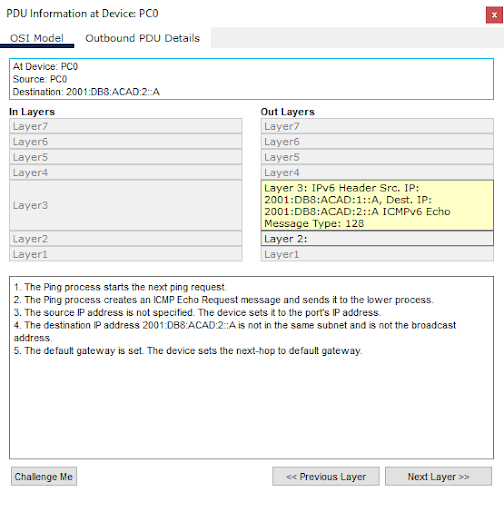
\includegraphics[width=0.7\textwidth]{../tpipv6/imagenes/imagen1}
\end{center}
 
 \textbf{(P4)} Se analizó el próximo evento NDP en pc0 y se observó que el ND es de tipo Neighbor solicitation (135) y la dirección IPv6 de origen es FE80::290:2BFF:FE89:2D86. Luego, IPv6 NDP determina la dirección de destino para reenviar el ICMPv6. Los siguientes mensajes NDP son parecidos las los mensajes de la sección anterior
 
 \textbf{(P5)} Luego, revisamos el siguiente mensaje ICMPv6 en pc0 y observamos
 
\begin{center}
	 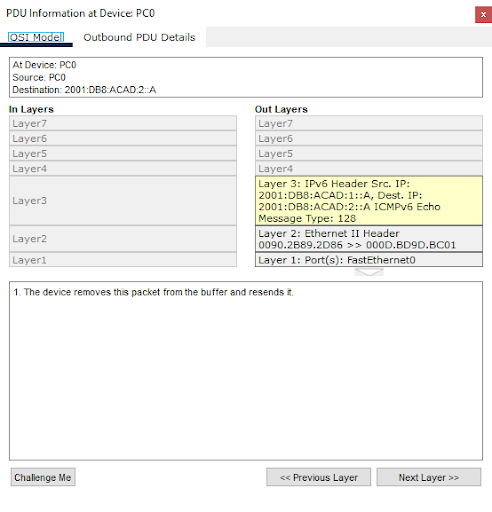
\includegraphics[width=0.7\textwidth]{../tpipv6/imagenes/imagen2}
\end{center}
 
 Como se puede observar, se posee información tanto de L3, ya que conoce las direcciones IPv6 de destino(router0) y de origen(pc0); como de L2, porque se conoce las direcciones MAC de origen(pc0) y de destino(router0) del paquete; por ende, tiene toda la información necesaria para enviar el mensaje. Las direcciónes MAC en la que está encapsulado el paquete es 0090.2B89.2D86 como dirección MAC de origen y 000D.BD9D.BC01 como dirección MAC de destino.
 
 \textbf{(P6)} Ahora analizamos el próximo evento ICMPv6 en R0
 
 \begin{center}
 	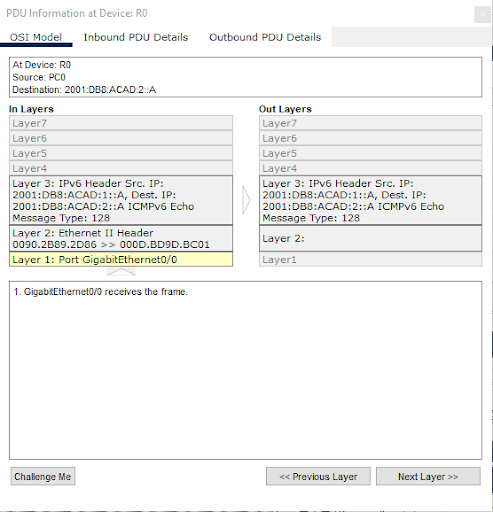
\includegraphics[width=0.7\textwidth]{../tpipv6/imagenes/imagen3}
 \end{center}
 
  Se puede observar que la PDU saliente del router no posee información de direcciones L2. ya que no tiene conocimiento sobrE las direcciones MAC de los dispositivos conectados a la LAN de la interfaz G0/0/1, por lo que tendrá que realizar una detección de vecinos en la red  2001:DB8:ACAD:2::
 
 \textbf{(P7)} Ahora, nos dirigimos al próximo evento ICMPv6 en PC2
 
 \begin{center}
 	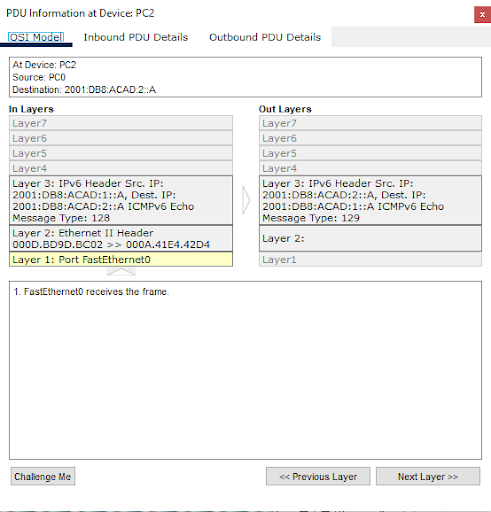
\includegraphics[width=0.7\textwidth]{../tpipv6/imagenes/imagen4}
 \end{center}
 
 como se puede observar, el mensaje ICMPv6 saliente de PC2 es de tipo Echo Reply (129), y como se puede observar, no contiene información de L2, ya que no reconoce la dirección MAC del router0 en el puerto G0/0/1 como default gateway
 
 \textbf{(P8)} Luego de realizar nuevamente un NDP de router0 a PC0, podemos observar que todas las direcciones se han aprendido, por lo que se PC2 puede enviar mensajes a PC0 sin problema.
 
 \textbf{(P9)} Reseteamos la simulación y volvemos a realizar un ping a PC2 desde PC0, se puede observar en el event list que no se realiza ningún NDP, ya que todos los dispositivos conocen las direcciones MAC de todos los involucrados en la comunicación.
 
 \textbf{(P10)} Revisamos la tabla de vecinos del router0 con show ipv6 neighbor y podemos observar que:
 
 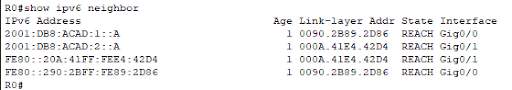
\includegraphics[width=0.7\textwidth]{../tpipv6/imagenes/imagen5}
 
 1-Aparecen en total 4 direcciones IPv6en la lista, 2 de GUA y 2 de Link Local Address.
 
 2-La dirección IGUA 2001:DB8:ACAD:1::A está asociada con PC0, al igual que la dirección LLA FE80::290:2BFF:FE89:2D86. La dirección GUA 2001:DB8:ACAD:2::A está asociada con PC2 al igual que la dirección LLA FE80::20A:41FF:FEE4:42D4.
 
 3-No hay ninguna entrada para PC1 en la lista debido a que no fue involucrado en la comunicación, por lo que router0 no tiene manera de saber de la existencia de PC1 y registrar su dirección MAC.
 
 \textbf{(P11)} si realizamos un ping desde router0 a PC1, podemos ver una modificación en la tabla:
 
 \begin{center}
 	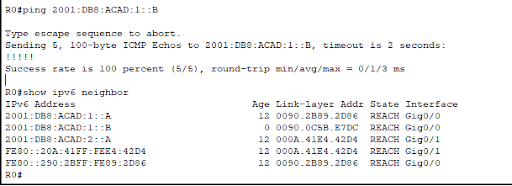
\includegraphics[width=0.7\textwidth]{../tpipv6/imagenes/imagen6}
 \end{center}
 
 Se puede observar que ahora el router conoce la dirección GUA PC1 y está agregado a su lista de vecinos. Si quisiera conocer también su dirección LLA, debería hacer ping a la LLA e ingresando el nombre del puerto por el que se realizará el ping.
 
 \begin{center}
 	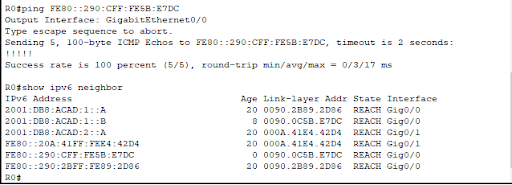
\includegraphics[width=0.7\textwidth]{../tpipv6/imagenes/imagen7}
 \end{center}
 
 Como se puede observar, ahora router0 conoce la dirección LLA de PC1, por que podemos decir, que ahora conoce todas las direcciones IPv6 de todos los dispositivos conectados a él.
 
 \section{Conclusiones}
 
 \begin{enumerate}
 	\item 
 	
 	\item 
 	
 	\item 
 	
 	\item 
 	
 	\item 
 	
 	\item 
 	
 \end{enumerate}
 
 \section{Referencias}
 Para la elaborcaión de este Trabajo de Investigación utilizamos estos videos:
 
  \begin{enumerate}
 	\item \textbf{“IPv6 SLAAC and EUI-64 Basics in Packet Tracer”}, by Dan Alberghetti, 2019, at https:
 	//www.youtube.com/watch?v=yMK1NVHksDE
 	
 	\item \textbf{“IPv6 NDP and ICMPv6 using Packet Tracer”} by Dan Alberghetti, 2020, at https://www.
 	youtube.com/watch?v=y2GpG9aOIFI
 	
 	\item \textbf{“Deteccion de vecinos IPv6 (Packet Tracer Lab 9.3.4)”} by RedesNetw channel, 2022, at
 	https://www.youtube.com/watch?v=ZBVXbgF39gw
 	
 \end{enumerate}
 
\end{document}
